\documentclass[9pt]{beamer}
% \documentclass[notes, handout, 9pt]{beamer}
% \documentclass[handout, 9pt]{beamer}

\usepackage{import}
\subimport{../}{preamble.tex}
\subimport{../}{beamer-theme.tex}
\usepackage{svg}

% Location for all figures / pictures
\graphicspath{{pictures/}{figures/}}

% % Figures inline
\usepackage{tikz}
\usepackage{pgfplots}
\usetikzlibrary{calc}
\usetikzlibrary{shapes.multipart}
\usetikzlibrary{decorations.pathreplacing}
\usetikzlibrary{arrows.meta}
\usepgfplotslibrary{fillbetween}

%--------------------------------------------------
% Presentation Information
%--------------------------------------------------
\title[Continuous Optimization]{Newton's Method}
\author[]{\textbf{Bart Van Parys}}
\date[]{Fall 2026}
%--------------------------------------------------

\begin{document}

\begin{frame}  

  \maketitle

  \vspace{-2em}
  
    \begin{center}
    \begin{tabular}{lll}
      Instructor : & \textbf{Bart Van Parys} & \textbf{(\href{mailto:mastermath@vanparys.xyz}{mastermath@vanparys.xyz})} \\
    \end{tabular}
  \end{center}
  
\end{frame}

\section{Newton's Method for Unconstrained Problems}

\begin{frame}{Gradient Method}

  Gradient Method
  \[
    x_{k+1} = x_k - h_k f'(x_k).
  \]

  \vfill
  
  Recall the reformulation of the gradient method
  \[
    x_{k+1 } \in \arg \min_{x} ~f(x_k) + \iprod{f'(x_k)}{x-x_k} + \frac{1}{2 h_k} \norm{x - x_k}^2_2. 
  \]

\end{frame}

\begin{frame}{Gradient Method}

  \begin{center}
    \begin{tikzpicture}
      
      \begin{axis}[
        ticks=none,
        axis lines=left,
        y=0.7cm,            % y unit vector
        x=1cm,            % x unit vector
        clip=true,
        xmin =-3,
        ymax=4,
        ymin=0,
        xlabel={ $\Re^n$},
        ylabel={ $f$},
        x label style={at={(axis description cs:0.9,0.05)},anchor=west},
        y label style={at={(axis description cs:0.25,1)},rotate=-90,anchor=south west},
        ]
        
        \addplot[mark=none, black, samples=100, domain=-4:4] { ln(exp(2*x) + exp(-2*x)) + 0.6/2*x^2};

        \node[circle, inner sep=0.75, fill=red] (x) at (axis cs:0.4, 1.0319) {};
        \node[right=0.2em] at (x) {\tiny $\bold x_k$};
        \only<2->{
          \addplot[ mark=none, red, samples=100, domain=-4:4] { 1.0319 + 1.56807*(x - 0.4) + 3*(x - 0.4)^2};
          \node[above] at (axis cs:-1.3,0) {{\color{red} \tiny $f(x_k)+\iprod{f'(x_k)}{x-x_k}$}};
          \addplot[ densely dotted, mark=none, red, samples=100, domain=-3:1.5] { 1.0319 + 1.56807*(x - 0.4)};
          \node[below] at (axis cs:0.1,4) {{\color{red} \tiny $+\frac{\norm{x-x_k}^2_2}{2h_k}$}};
        }

        \only<3->{
          \node[circle, inner sep=0.75, fill=red] (xp) at (axis cs:0.15287, 0.826996) {};
          \node[below=0.2em] at (xp) {\tiny $\bold x_{k+1}$};
        }

      \end{axis}
      
    \end{tikzpicture}
  \end{center}


\end{frame}

\begin{frame}{Using the Best Quadratic Approximation : Newton Method}


  Consider
  \[
    x_{k+1 } \in \arg \min_{x} f(x_k) + \iprod{f'(x_k)}{x-x_k} + \frac{1}{2} \iprod{f''(x_k)(x - x_k)}{x - x_k}
  \]
  in which we substituted the matrix $\mb I_n/h_k$ with the Hessian $f''(x_k)$.

  \vfill

  \emph{Newton's Method :} (when $f''(x_k)\succ 0$)
  \begin{center}
    \begin{tcolorbox}[width=0.7\textwidth]
      \[
        x_{k+1} \defn x_k - f''(x_k)^{-1} f'(x_k)
      \]
    \end{tcolorbox}
  \end{center}

\end{frame}

\begin{frame}{Newton's Method}
  \begin{center}
    \begin{tikzpicture}
      
      \begin{axis}[
        ticks=none,
        axis lines=left,
        y=0.7cm,            % y unit vector
        x=1cm,            % x unit vector
        clip=true,
        xmin =-2,
        ymax=4,
        ymin=0,
        xlabel={ $\Re^n$},
        ylabel={ $f$},
        x label style={at={(axis description cs:0.9,0.05)},anchor=west},
        y label style={at={(axis description cs:0.25,1)},rotate=-90,anchor=south west},
        ]
        
        \addplot[mark=none, black, samples=100, domain=-4:4] { ln(exp(2*x) + exp(-2*x)) + 0.6/2*x^2};

        \node[circle, inner sep=0.75, fill=red] (x) at (axis cs:0.4, 1.0319) {};
        \node[right=0.2em] at (x) {\tiny $\bold x_k$};
        \only<2->{
          \addplot[ mark=none, red, samples=100, domain=-4:4] { 1.0319 + 1.56807*(x - 0.4) + 1.41811*(x - 0.4)^2};
        }

        \only<3->{
          \node[circle, inner sep=0.75, fill=red] (xp) at (axis cs:-0.15287, 0.59843) {};
          \node[below=0.2em] at (xp) {\tiny $\bold x_{k+1}$};
        }
      \end{axis}
      
    \end{tikzpicture}
  \end{center}
\end{frame}

\begin{frame}{Newton's Method Has Disadvantages}

  \begin{itemize}
    \setlength\itemsep{1em}
  \item Oracle : $x\mapsto (f'(x) , f''(x))$
  \item The Hessian should be invertible
  \item As such not applicable to constrained problems
  \item Expensive if $f''(x)$ is a dense matrix
  \end{itemize}

  \vfill

  What about the \emph{convergence} ?
  
\end{frame}

\begin{frame}{Example I}

  \begin{center}
    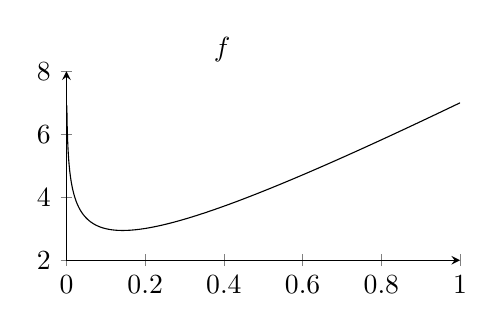
\begin{tikzpicture}
      
      \begin{axis}[
        %ticks=none,
        axis lines=left,
        y=0.4cm,            % y unit vector
        x=5cm,            % x unit vector
        clip=true,
        xmin =0,
        xmax =1,
        ymax=8,
        ymin=2,
        %xlabel={ $\Re$},
        ylabel={ $f$},
        x label style={at={(axis description cs:0.9,0.05)},anchor=west},
        y label style={at={(axis description cs:0.35,1)},rotate=-90,anchor=south west},
        ]
        
        \addplot[mark=none, black, samples=1000, domain=0:1] { 7*x-ln(x)};

      \end{axis}
      
    \end{tikzpicture}
  \end{center}

  \vfill
  
  \begin{itemize}
    \setlength\itemsep{1em}
  \item Convex function $f(x)=7x-\log x$ with minimizer $x^*=\frac{1}{7}=0.142857143$.
  \item Gradient $f'(x)=7-\frac{1}{x}$.
  \item Hessian $f''(x)=\frac{1}{x^2}$.
  \end{itemize}

\end{frame}

\begin{frame}{Computation}
  \begin{center}
    \begin{tabular}{|c||c||c||c|}
       \hline
       $k$ & $x_k$  &$x_k$ &$x_k$ \\ \hline
       0 & 1 &  0.01 & 0.1 \\
       1 & \red{-5}  & 0.0193 & 0.13 \\
       2 &  &  0.03599 & 0.1417 \\
       3 &  &  0.062917 & 0.14284777 \\
       4 &  &  0.098124 & 0.142857142\\
       5 &  &  0.128849782 &0.142857143\\
       6 & &  0.141483700 & 0.142857143\\
       7 & &  0.142843938 & 0.142857143\\
       8 & &  0.142857142 & 0.142857143\\\hline
     \end{tabular}
 \end{center}

 \vfill
 
 \textbf{Remarks:}
 \begin{itemize}
 \item When $\bold x_0\approx \bold x^\star$, then Newton's method converges.
 \item Failure I : If $\bold x_0 \not\approx \bold x^\star$, then Newton's method can fail to be defined.
 \end{itemize}
\end{frame}

\begin{frame}{Example II}

  \begin{center}
    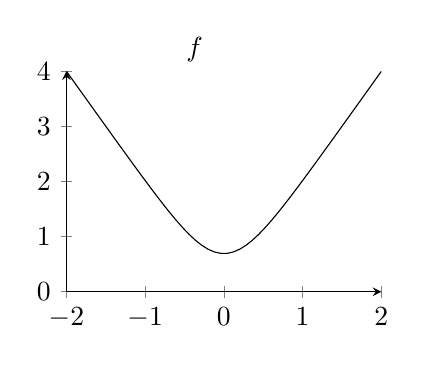
\begin{tikzpicture}
      
      \begin{axis}[
        %ticks=none,
        axis lines=left,
        y=0.7cm,            % y unit vector
        x=1cm,            % x unit vector
        clip=true,
        xmin =-2,
        xmax =2,
        ymax=4,
        ymin=0,
        %xlabel={ $\Re^n$},
        ylabel={ $f$},
        x label style={at={(axis description cs:0.9,0.05)},anchor=west},
        y label style={at={(axis description cs:0.35,1)},rotate=-90,anchor=south west},
        ]
        
        \addplot[mark=none, black, samples=100, domain=-4:4] { ln(exp(2*x) + exp(-2*x)) };
      \end{axis}
      
    \end{tikzpicture}
  \end{center}

  \vfill
  
  \begin{itemize}
    \setlength\itemsep{1em}
  \item Convex function $f(x)=\log(\exp(2 x) + \exp(-2 x))$ with minimizer $x^*=0$.
  \item Gradient $f'(x)=\tfrac{2 (\exp(4 x) - 1)}{(\exp(4 x) + 1)}$.
  \item Hessian $f''(x)=\tfrac{16 \exp(4 x)}{(\exp(4 x) + 1)^2}$.
  \end{itemize}
\end{frame}

\begin{frame}{Computation}
  \begin{center}
    \begin{tabular}{|c||c||c|}
       \hline
       $k$ & $x_k$  &$x_k$ \\ \hline
       0 & 0.6 &  0.5  \\
       1 & -0.766557  & -0.406715  \\
       2 & 1.91022 &  0.204701  \\
       3 & -258.288 &  -0.0236525  \\
       4 & \red{``Inf''} &  $3.53014\e{-5}$ \\
       5 &  &  $-1.17306\e{-13}$ \\
       6 & &  $-1.1418\e{-17}$ \\\hline
     \end{tabular}
 \end{center}

 \vfill
 
 \textbf{Remarks:}
 \begin{itemize}
 \item When $\bold x_0\approx \bold x^\star$, then Newton's method converges.
 \item Failure II : If $\bold x_0 \not\approx \bold x^\star$, then Newton's method can diverge.
 \end{itemize}
\end{frame}

\begin{frame}{Convergence is much faster}

  \begin{minipage}{0.7\textwidth}
    Let $f:\Re^n\to\nRe$ satisfy
    \begin{itemize}
      \setlength\itemsep{1em}
    \item $f$ is twice differentiable
    \item $f''(x^\star) \succeq_{S^n_+} \ell \cdot \mb I_n \succ 0$
    \item The Hessian $f''$ is Lipschitz continuous w.r.t.\ $\norm{\cdot}_2$, i.e.,
      \[
        \norm{f''(x) -f''(y)} \leq M \norm{x-y}_2
      \]
      where $\norm{A} = \sup_{\norm{x}_2\leq 1} \norm{A x}_2 = \max_i \abs{\lambda_i(A)}$.
    \end{itemize}    
  \end{minipage}%
  \hfill
  \begin{minipage}{0.3\textwidth}
    \centering
    
\includegraphics[height=3cm]{kantorovich.jpg}
  \end{minipage}

  \vfill
  
  \textbf{Theorem :} If $\norm{x_0-x^\star}_2 \leq \frac{2\ell}{3 M}$, then the iterates $x_k$ of Newton's method are \emph{well-defined}, satisfy
  \begin{align*}
    \norm{x_{k+1}-x^\star}_2 \leq \frac{M \norm{x_k-x^\star}_2^2}{2 \left( \ell - M \norm{x_k-x^\star}_2\right)}& \leq \norm{x_{k}-x^\star}_2 \\[0.5em]
    & \leq \frac{3M}{2 \ell} \norm{x_k-x^\star}_2^\emph{2}.
  \end{align*}
\end{frame}

\begin{frame}{Drawing}

  \begin{center}
    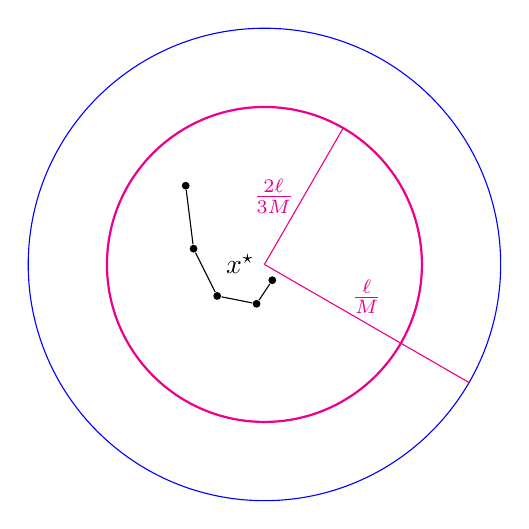
\begin{tikzpicture}
      \draw [magenta, thick] circle [radius=2];
      \draw [blue] circle [radius=3];

      \draw [magenta] (0,0) -- node[left,magenta] {$\frac{2\ell}{3M}$} (60:2);
      \node [left] at (0, 0) {$x^\star$};

      \draw [magenta] (0,0) -- node[above,magenta] {$\frac{\ell}{M}$} (-30:3);

      \node [fill=black,inner sep=1, circle] (x0) at (-1, 1) {};
      \node [fill=black,inner sep=1, circle] (x1) at (-0.9, 0.2) {};
      \node [fill=black,inner sep=1, circle] (x2) at (-0.6, -0.4) {};
      \node [fill=black,inner sep=1, circle] (x3) at (-0.1, -0.5) {};
      \node [fill=black,inner sep=1, circle] (x4) at (0.1, -0.2) {};

      \draw (x0)--(x1);
      \draw (x1)--(x2);
      \draw (x2)--(x3);
      \draw (x3)--(x4);

    

    
  \end{tikzpicture}
\end{center}

\end{frame}

\begin{frame}{Kantorovich's Proof}

  
  \textbf{Proof : (induction)}

  \begin{itemize}
  \item (trivial) Let $r_k \defn \norm{x_k-x^\star}_2$ for every $k$. Now $f''(x_k) -f''(x^\star) \succeq -M \norm{x_k-x^\star}_2 \mb I_n$ and hence $f''(x_k) \succeq (\ell - M r_k) \mb I_n$.  Iterates are well defined when $r_k < \tfrac{\ell}{M}$. First iterate $x_0$ with $r_0 <  \tfrac{2\ell}{(3M)}<\tfrac{\ell}{M}$  has well defined Newton step.\\[1em]
  \item (induction) we have that when $r_k < \tfrac \ell M$:
    \begin{align*}
      x_{k+1} - x^\star & = x_k - x^\star - f''(x_k)^{-1} f'(x_k)\\
                        & = f''(x_k)^{-1} \left( f''(x_k) (x_k - x^\star) - (f'(x_k)-f'(x^\star))  \right)\\
                        & = f''(x_k)^{-1} \left( \int_0^1 \left[ f''(x_k) - f''(x^\star + t (x_k - x^\star)) \right] (x_k - x^\star) dt \right)
    \end{align*}
    which implies
    \begin{align*}
      r_{k+1} & \leq \norm{f''(x_k)^{-1}}_2 \left( \int_0^1 \norm{f''(x_k) - f''(x^\star + t (x_k - x^\star))}\d t \right) r_k\\
              & \leq \norm{f''(x_k)^{-1}}_2 \frac{M}{2} r^2_k\leq \frac{M r_k^2}{2 (\ell - M r_k)} \leq \frac{3M}{2\ell} r_k^2. 
    \end{align*}
    Note that $r_{k+1} < r_k$ when $r_k< \tfrac{2\ell}{(3 M)}$ because then $\tfrac{M r_k^2}{(2 (\ell-M r_k))} < r_k$.

  \end{itemize}
\end{frame}

\begin{frame}{Newton's method has disadvantages}

  \begin{itemize}
    \setlength\itemsep{1em}
  \item Oracle : $x\mapsto (f(x), f'(x) , f''(x))$
  \item The Hessian should be invertible
  \item As such not applicable to constrained problems
  \item Expensive if $f''(x)$ is a dense matrix
  \end{itemize}

  \vfill

  What about the \emph{convergence} ?
  \begin{itemize}
    \setlength\itemsep{1em}
  \item Convergence is much faster $N = \mc O(\log\log(\frac 1\epsilon))$, \textbf{but only local}!!
  \item The theory of \emph{self-concordant functions} shows quite exactly how Newton's method can be used at best.
  \end{itemize}
  
\end{frame}

\begin{frame}{Newton's Method is Affine Invariant}


  
  \begin{minipage}{0.5\textwidth}

    Optimization Problem
    \[
      \begin{array}{rl}
        \min_{x\in \Re^n} & f(x)
      \end{array}
    \]

    \vfill

    Newton Iterates
    \[
      \begin{array}{rl}
        x_0 & = \bar x \\[0.5em]
              x_{k+1} & = x_k - f''(x_k)^{-1}f'(x_k)
      \end{array}
    \]

    \vfill

    \centering
    \includesvg[height=2.5cm]{conv1.svg}
  \end{minipage}%
  \hfill
  \begin{minipage}{0.5\textwidth}

    Optimization Problem
    \[
      \begin{array}{rl}
        \min_{y\in \Re^n} & \phi(y)\defn f(A y)
      \end{array}
    \]

    \vfill

    Newton Iterates
    \[
      \begin{array}{rl}
        y_0 & = A^{-1} \bar x \\[0.5em]
        y_{k+1} & = y_k - \phi''(y_k)^{-1}\phi'(y_k)
      \end{array}
    \]

    \vfill
    
    \centering
    \includesvg[height=2.5cm]{conv2.svg}
  \end{minipage}
  \vfill

  Invariance:
  \[
    \red{x_k\qquad=\qquad Ay_{k}}
  \]
\end{frame}

% \begin{frame}{Drawing}
% \end{frame}

\begin{frame}{Newton's Method is Affine Invariant [$\star$]}

  Let $f$ be a twice differentiable function. Change of variables $x = A y$ with $A$ an invertible matrix. Then, $$\red{y_k = A^{-1} x_k}$$ for all $k$ for which $x_k$ exists.

  \vfill

  \textbf{Proof :}
  \begin{itemize}
  \item We have gradient $\phi'(y) = A\tpose f'(A y)$ as
    \[
      \iprod{\phi'(y)}{h} \defn \lim_{t\downarrow 0} \frac{f(A (y+t h)) - f(A y)}{t} = \iprod{f'(Ay)}{Ah} = \iprod{A\tpose f'(A y)}{h}.
    \]
  \item Similarly, one can show that $\phi''(y) = A\tpose f''(Ay) A$, which exists if and only if $f''(Ay)$ exists.
  \item Thus,
    \[
      y_{k+1} = y_k - (A\tpose f''(A y_k) A)^{-1} A\tpose f'(A y_k) = y_k - A^{-1} f''(A y_k)^{-1} f'(A y_k).
    \]
    Induction on $k$ gives the final result.
  \end{itemize}
\end{frame}


\begin{frame}{Kantorovich's Convergence Result is Not Affine Invariant !?}

  \begin{minipage}{0.7\textwidth}
    Let $f:\Re^n\to\nRe$ satisfy
    \begin{itemize}
    \item $f$ is twice differentiable
    \item $f''(x^\star) \succeq \ell \cdot \mb I_n \succ 0$
    \item The Hessian $f''$ is Lipschitz continuous w.r.t.\ $\norm{\cdot}_2$, i.e.,
      \[
        \norm{f''(x) -f''(y)}\leq M \norm{x-y}_2
      \]
      where $\norm{A} = \sup_{\norm{x}_2\leq 1} \norm{A x}_2 = \max_i \abs{\lambda_i(A)}$.
    \end{itemize}    
  \end{minipage}%
  \hfill
  \begin{minipage}{0.3\textwidth}
    \centering
    
\includegraphics[height=3cm]{kantorovich.jpg}
  \end{minipage}

  \vfill
  
  \textbf{Theorem :} If \red{$\norm{x_0-x^\star}_2 \leq \frac{2\ell}{3 M}$}, then the iterates $x_k$ of Newton's method are \emph{well-defined} and
  \[
    \red{\Vert} x_{k+1}-x^\star \red{\Vert}_{\red{2}} \leq \frac{M \red{\Vert} x_k-x^\star \red{\Vert_2}^2}{2 \left( \ell - M \red{\Vert} x_k-x^\star \red{\Vert_2}\right)}\leq \frac{3M}{2 \ell} \red{\Vert} x_k-x^\star \red{\Vert_2}^2.
  \]
  
\end{frame}

\begin{frame}{How to Correct Kantorovich's Result ?}

  Let $f:\Re^n\to\nRe$ satisfy
  \begin{itemize}
    \setlength\itemsep{1em}
  \item $f$ is twice differentiable
  \item $f''(x^\star) \succeq \ell \cdot \mb I_n \succ 0$
  \item \red{The Hessian $f''$ is Lipschitz continuous w.r.t.\ $\norm{\cdot}_2$, i.e.,
      \[
        \norm{f''(x) -f''(y)}_2\leq M \norm{x-y}_2
      \]
      where $\norm{A} = \sup_{\norm{x}_2\leq 1} \norm{A x}_2 = \max_i \abs{\lambda_i(A)}$.}
  \end{itemize}
  The last condition is not affine-invariant because of the \red{norm}.

  \vfill

  \textbf{The solution of Nesterov and Nemirovski:} Use the norm $\norm{h}_x\defn \sqrt{\iprod{f''(x) h}{h}}$.\\[1em]

  Remark :
  \begin{itemize}
  \item $\norm{h}_x = \sqrt{\iprod{\phi''(y) A^{-1} h}{A^{-1} h}}$ where $\phi(y) = f(Ay)$
  \item $\norm{h}_{x, \star} = \sqrt{\iprod{f''(x)^{-1} h}{h}}$
  \end{itemize}
  
  
  
\end{frame}

\section{Constraints and Newton's Method}

\begin{frame}{Dealing with Equality Constraints}

  Let $f:\Re^n\to\nRe$ be a twice differentiable convex function.\\
  \emph{Equality constrained} convex optimization problem:
  \[
    \begin{array}{rl}
      \min_{x\in\Re^n} & f(x) \\[1em]
      \st & \blue{A x=b}
    \end{array}
  \]
  
  \begin{itemize}
  \item Equality constraints for convex problems must be linear.
  \item Without loss of generality : $A\in\Re^{m\times n}$ has full row rank.
  \end{itemize}

\end{frame}

\begin{frame}{Constraint Newton Method}

  \begin{center}
    \begin{tikzpicture}
      
      \begin{axis}[
        ticks=none,
        axis lines=left,
        y=0.7cm,            % y unit vector
        x=1cm,            % x unit vector
        clip=true,
        xmin =-2,
        ymax=4,
        ymin=0,
        xlabel={ $\Re^n$},
        ylabel={ $f$},
        x label style={at={(axis description cs:0.9,0.05)},anchor=west},
        y label style={at={(axis description cs:0.25,1)},rotate=-90,anchor=south west},
        ]
        
        \addplot[mark=none, black, samples=100, domain=-4:4] { ln(exp(2*x) + exp(-2*x)) + 0.6/2*x^2};

        \node[circle, inner sep=0.75, fill=red] (x) at (axis cs:0.4, 1.0319) {};
        \node[right=0.2em] at (x) {\tiny $\bold x_k$};
        \only<2->{
          \addplot[ mark=none, red, samples=100, domain=-4:4] { 1.0319 + 1.56807*(x - 0.4) + 1.41811*(x - 0.4)^2};
        }

        \only<3->{
          \node[circle, inner sep=0.75, fill=red] (xp) at (axis cs:-0.15287, 0.59843) {};
          \node[below=0.2em] at (xp) {\tiny $\bold x_{k+1}$};
        }
      \end{axis}
      
    \end{tikzpicture}
  \end{center}

  \vfill
  
  Newton iteration:
  \[
    \begin{array}{rl}
       x_{k+1} \in \arg \min & f( x_k) + f'( x_k)'( x- x_k) + \frac{1}{2} ( x -  x_k)' f''( x_k)( x -  x_k)\\[0.5em]
      \st &  A  x= b
    \end{array}
  \]

  \textbf{Observations:}
  \begin{itemize}
  \item Quadratic minimization over an affine subspace
  \item<4-> Closed form solvable!
  \end{itemize}
  
\end{frame}


\begin{frame}{Newton's Method}

  
  
  \textbf{Theorem:} Newton's method iterate $ x_{k+1}$ solves
  \[
    \begin{pmatrix}
      f''( x_k) &  A ' \\
       A &  0%_{m\times n}
    \end{pmatrix}
    \begin{pmatrix}
       x_{k+1}\\
       p_{k+1}
    \end{pmatrix}
    =
    \begin{pmatrix}
      f''( x_k) x_k - f'( x_k)\\
       b
    \end{pmatrix}.
  \]
  Furthermore, if $f''( x_k) \succ 0$, then the Newton system is \emph{uniquely} defined.

  \vfill

  \textbf{Proof :}
  
  \begin{itemize}
  \item<2-> We show that 
    \[
      \begin{pmatrix}
        f''( x_k) &  A ' \\
         A &  0%_{m\times n}
      \end{pmatrix}
      \begin{pmatrix}
         x\\
         p
      \end{pmatrix}
      =
      \begin{pmatrix}
         0\\
         0
      \end{pmatrix}.
    \]
    admits only the trivial solution.
  \item<3-> Taking the scalar product of the first equation with $ x$ gives
    \[
       x' f''( x_k) x +   x'  A'  p =  x' f''( x_k) x = 0,
    \]
    and hence $ x= 0$.
  \item<4-> Now $ A'  p =  0 \iff  p =  0$ as $ A$ has full row rank.
    % Null space of the considered system is $\{ 0\}$.
  \end{itemize}
  
\end{frame}

\begin{frame}{The Null Space Method -- Reduction to an Unconstrained Problem}


  \uncover<2->{
  \textbf{Nullspace representation:} we have
  \[
    \set{x\in\Re^n}{Ax=b} = \set{Bp +\tilde x}{p\in \Re^{n-m}}
  \]
  for some matrix $B\in \Re^{n\times{(n-m)}}$ and $\tilde x\in\Re^n$ with $A\tilde x=b$. We have $\rm{span}(B)=\rm{null}(A)$.
  }

  \vfill
  
  \begin{minipage}{0.45\textwidth}

    Optimization Problem
    \[
      \begin{array}{rl}
        \min_{x\in \Re^n} & f(x) \\
        \st & Ax = b
      \end{array}
    \]

    \vfill

    Newton Iterates
    \[
      \begin{array}{rl}
        x_0 & = \bar x \\[0.5em]
        x_{k+1} & =\rm{constraint~Newton}
      \end{array}
    \]

  \end{minipage}%
  \hfill
  \uncover<3->{%
  \vrule
  \hfill
  \begin{minipage}{0.45\textwidth}

    Optimization Problem
    \[
      \begin{array}{rl}
        \min & \phi(p)\defn f(Bp + \tilde x) \\
        \st & p\in \Re^{n-m}
      \end{array}
    \]

    \vfill

    Newton Iterates
    \[
      \begin{array}{rl}
        B p_0 + \tilde x & = \bar x \\[0.5em]
        p_{k+1} & = p_k - \phi''(p_k)^{-1}\phi'(p_k)
      \end{array}
    \]
  \end{minipage}
}
  \vfill

 \uncover<4-> {
  \textbf{Theorem} (Invariance): We have
  \(
    \red{x_k  = Bp_k+\tilde x}
  \)
  for all $k$.
  }
\end{frame}

\begin{frame}{Proof [$\star$]}

  \begin{itemize}
  \item (Trivial case) We have that $x_0 = B p_0 + \tilde x$
  \item<2-> (Induction) The induction hypothesis is $x_k=B p_k+\tilde x$. Newton updates 
    \begin{align*}
      \{x_{k+1}\} = & \arg\min_{Ax=b} f(x_k)+ \iprod{f'(x_k)}{x-x_k} + \frac 12 \iprod{f''(x_k)(x-x_k)}{(x-x_k)},\\[0.5em]
      \{p_{k+1}\} = & \arg\min_{p} ~ \phi(p_k)+ \iprod{\phi'(p_k)}{p-p_k} + \iprod{\phi''(p_k)(p-p_k)}{(p-p_k)}/2 \\[0.5em]
                 =   & \arg\min_{p} ~ f(Bp_k+\tilde x)+ \iprod{f'(Bp_k+\tilde x)}{B(p-p_k)}\\[-0.35em]
                    &\hspace{8.4em} + \iprod{f''(Bp_k+\tilde x)B (p-p_k)}{B (p-p_k)}/2 \\[0.5em]
      = & \arg\min_{p} ~ f(x_k)+ \iprod{f'(x_k)}{Bp+\tilde x-x_k)} \\[-0.35em]
                    & \hspace{8.4em} + \iprod{f''(x_k)(Bp+\tilde x-x_k)}{Bp+\tilde x-x_k}/2 
    \end{align*}
  \item<3-> As we have that $\set{x\in\Re^n}{Ax=b} = \set{Bp +\tilde x}{p\in \Re^{n-m}}$ it follows that $x_{k+1} = Bp_{k+1}+\tilde x$.
  \end{itemize}
  
  
% :}
    
%     = & \arg\min_{p} \iprod{f'(B p_k+x_0)}{B(p-p_k)} + \frac 12 \iprod{ f''(B p_k+x_0)B (p-p_k)}{B(p-p_k)} 
%   \end{align*}
%   The $p_{k}$ are precisely the Newton iterates for the unconstrained problem $\min_{p} f(Bp+x_0)$. 

\end{frame}

\begin{frame}{The Null Space Method -- Reduction to an Unconstrained Problem}

  Remarks:
  \begin{itemize}
  \item Null space method produces the same iterates as the constrained Newton's method.
  \item Indirectly proves its convergence.
  \end{itemize}
  
\end{frame}

\section{Sequential Quadratic Optimization}


\begin{frame}{Sequential Quadratic Optimization}

  General optimization problem:
  \[
    \begin{array}{rl}
      \min_{x} & f(x) \\[0.5em]
      \st & g_i(x) = 0 \quad \forall i\in [1, \dots, m] \\ 
    \end{array}
  \]

  \vfill
  
  Exploiting the idea of equality constrained Newton method:
  \[
    \begin{array}{rl}
      x_{k+1} =\arg \min_{x} & f(x_k) + \iprod{f'(x_k)}{x-x_k}+\frac 12 \iprod{f''(x_k)(x-x_k)}{x-x_k} \ \\[0.5em]
      \st & g_i(x_k) + \iprod{g_i'(x_k)}{x-x_k} = 0 \quad \forall i\in [1, \dots, m] \\
    \end{array}
  \]

  \vfill

  \textbf{Remarks:}
  \begin{itemize}
  \item Works very well in practice
  \item Iterates are not necessarily feasible
  \item Convergence is technical to prove and not global
  \item We will study barrier methods instead
  \end{itemize}
  
\end{frame}


\end{document}
%%% Local Variables:
%%% mode: latex
%%% TeX-master: t
%%% End:
